\section{Unsupervised persona exploration}\label{sec:unsupervised-persona-exploration}
We find four interpretable persona axes in Llama-3.1-8B-Instruct that are stable within-model and partially replicate across model families; we then evaluate the extent to which they can be modulated by LoRA adapters trained with the supervised pipeline of \Cref{sec:supervised}.
We do not expect that all LLM behaviour will be explainable by human-derived (e.g.\ OCEAN) traits.
\david{
We therefore ask whether persona axes can be discovered directly from model
behaviour, and test whether a psychometric-style pipeline can recover
stable, interpretable latent factors from a population of model rollouts. This
provides a route from human-specified trait control toward model-native persona
discovery.
}

\textbf{A population of personas is produced by generating diverse rollouts.}
In \david{traditional psychometrics} it is typical to sample across a large population size, with the variation across this population being the object of study.
This does not translate nicely to the case of LLMs by sampling different post-trained models, in part because there are fewer LLMs than humans, and in part because the `persona' depends on the context.
However, this last point can be used to our advantage: \david{a single model can express different behavioural dispositions under different contexts.}
We sample 2{,}500 15-turn rollouts from Llama-3.1-8B-Instruct, with each rollout's interlocutor (gpt-5.4-nano) randomly assigned one of 25 conversational archetypes and one of 100 scenario scripts.
\david{This design follows the ``weights plus context'' view of personas introduced above. The model weights define the behavioural repertoire, while the context selects a region of that repertoire. By sampling many contexts, we obtain a population over which latent behavioural structure can be estimated.}

\textbf{Exploratory latent factors are discovered using responses to a forced-choice questionnaire.}
For each persona-rollout we produce an $(N{+}1)$th-turn generation of one of two contrasting first-person continuations for each of 72 forced-choice items, and read the per-letter logprobs as the response.
We use Horn's parallel analysis to inform the number of factors and retain $k=4$ at the scree elbow (Appendix~\ref{sec:appendix-fa-validation}); the fit is principal axis factoring with oblimin rotation, allowing correlated factors.

\textbf{We find four factors that are interpretable, stable within-model, and partially replicated across models.}
The factor loadings are inspected (using LLM-labellers, with manual human inspection to corroborate and augment labeller output against the highest- and lowest-loading items) to produce human-understandable axis names.
The four factors are: \textit{Initiative} (proactive volunteering vs literal compliance), \textit{Warmth} (playful tonal mirroring vs formal detachment), \textit{Pedagogy} (structured explanatory mode vs casual minimalism), and \textit{Hedging} (epistemic caution vs confident conviction).
Cronbach's $\alpha$ ranges $0.72$--$0.87$ across factors and models, and per-factor split-half congruence exceeds $|\phi|=0.97$ on every factor on both models, supporting within-model stability (Appendix~\ref{sec:appendix-fa-validation}).
Administering the same questionnaire with Qwen2.5-7B-Instruct on the same Llama rollouts yields four factors whose Hungarian-matched per-pair Tucker's $|\phi|$ averages $0.66$ on shared items, with \textit{Warmth} the strongest cross-model match at $|\phi|=0.80$ (Appendix~\ref{sec:appendix-fa-validation}).
Conversational-scenario assignment alone explains $56$--$78\%$ of each factor's score variance, but three of four factors (\textit{Initiative}, \textit{Warmth}, \textit{Hedging}) survive a scenario-residualized refit at $|\phi| \in [0.89, 0.94]$; \textit{Pedagogy} is the most scenario-dependent at $|\phi|=0.69$ (Appendix~\ref{sec:appendix-fa-residualized}).
For full per-factor item details, see \Cref{sec:appendix-fa-factors}.

\textbf{Modifying these factors using the supervised LoRA approach of \Cref{sec:supervised} succeeds clearly for one factor and partially for the other.}
We trained four LoRAs covering the top two factors by variance explained --- \{\textit{Initiative}, \textit{Warmth}\} $\times$ \{amplifier, suppressor\} --- and re-administered the questionnaire under each adapter to a held-out subsample of personas\footnote{Constitutions were carefully crafted and checked to ensure no appearance of any actual questionnaire items, to avoid validation leakage.}.
Figure~\ref{fig:4-lora-shifts} shows the per-LoRA per-factor mean shift in factor-score units, restricted to the medium tertile of baseline score on each column factor: this restriction reports the LoRA's effect on a typical neutral-baseline persona, avoiding the ceiling/floor effects that bias the full-sample mean toward zero on personas already saturated near the high or low pole.
The full-sample (naive) and headroom-conditioned views, which tell a quantitatively similar story, are reported in Appendix~\ref{sec:appendix-fa-lora-shifts}.
\textit{Initiative}-amplifier produces a clean on-target effect ($+1.5\sigma$ in factor-score units, rising to $+1.8\sigma$ on personas with most baseline headroom), while the \textit{Warmth} LoRAs show weaker target effects and substantial spillover onto neighbouring axes (most notably onto \textit{Hedging}).
We read the partial successes as a mix of weak factor identification, training-data leakage to neighbouring axes, and constitution-curation artefacts (Appendix~\ref{sec:appendix-fa-lora-shifts}).

% Generated by: scripts_dev/unsupervised_embeddings/analysis_for_paper.v2.py
% Data: persona-shattering-lasr/monorepo @ fine_tuning/llama-3.1-8b-it/unsupervised/{initiative,warmth}/{amplifier,suppressor}/vunsup_k4_v7_pf3_paired_dpo/evals/factor_validate/
\begin{figure}[htbp]
\centering
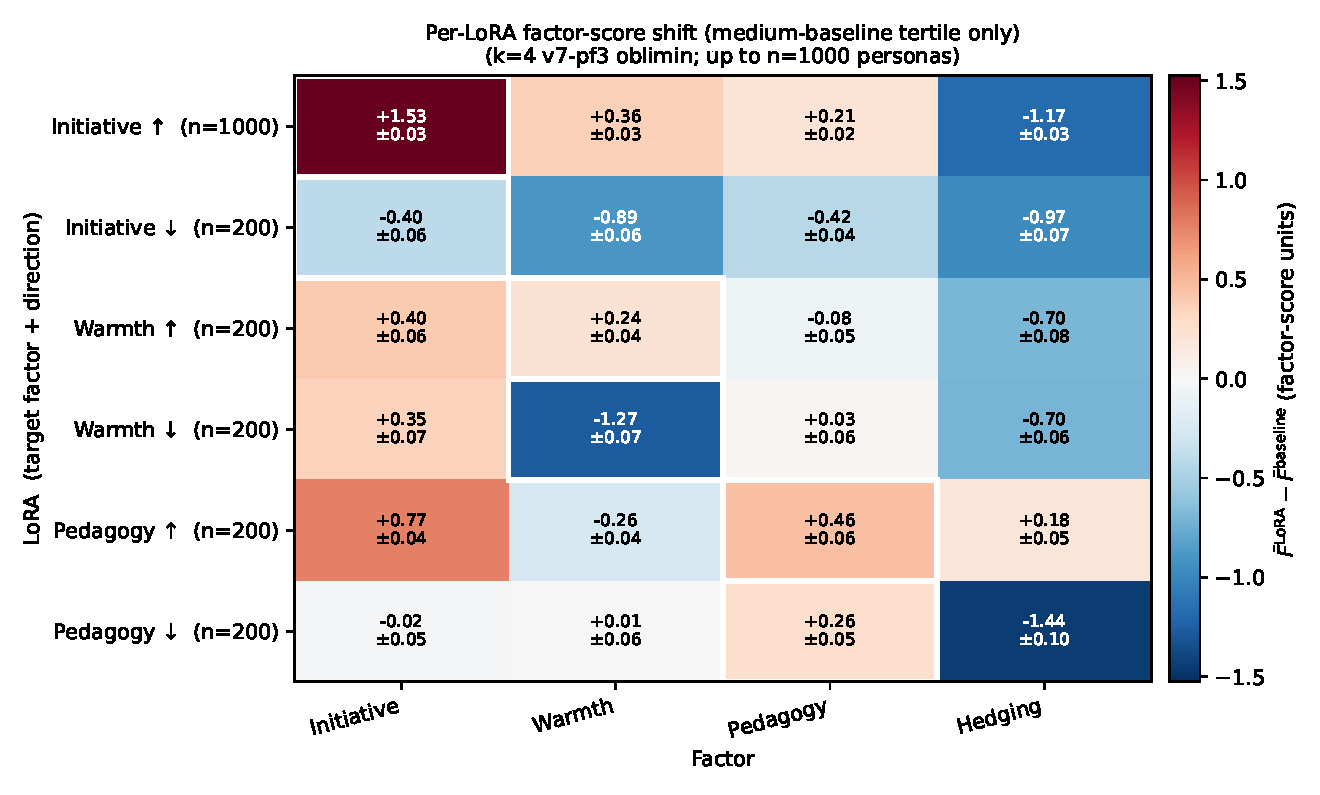
\includegraphics[width=\linewidth]{figures/unsupervised/fig_4_2_6b_lora_shifts_middling.pdf}
\caption{Per-LoRA mean factor-score shift, restricted to the medium tertile of baseline score on each column factor (the typical neutral-baseline persona). Rows are trained LoRAs (target factor and direction); columns are the four recovered factors. Cell values are $\Delta = \bar{F}^{\text{LoRA}} - \bar{F}^{\text{baseline}}$ in factor-score units, with the half-width of the 95\% bootstrap CI underneath. White outlines mark each LoRA's intended (target factor, direction) cell. \textit{Initiative}-amplifier uses $n=1000$ validation personas; the others use $n=200$. Naive and headroom views are reported in Appendix~\ref{sec:appendix-fa-lora-shifts}.}
\label{fig:4-lora-shifts}
\end{figure}
